\documentclass[final,t]{beamer}\usepackage[]{graphicx}\usepackage[]{color}
% maxwidth is the original width if it is less than linewidth
% otherwise use linewidth (to make sure the graphics do not exceed the margin)
\makeatletter
\def\maxwidth{ %
  \ifdim\Gin@nat@width>\linewidth
    \linewidth
  \else
    \Gin@nat@width
  \fi
}
\makeatother

\definecolor{fgcolor}{rgb}{0.345, 0.345, 0.345}
\newcommand{\hlnum}[1]{\textcolor[rgb]{0.686,0.059,0.569}{#1}}%
\newcommand{\hlstr}[1]{\textcolor[rgb]{0.192,0.494,0.8}{#1}}%
\newcommand{\hlcom}[1]{\textcolor[rgb]{0.678,0.584,0.686}{\textit{#1}}}%
\newcommand{\hlopt}[1]{\textcolor[rgb]{0,0,0}{#1}}%
\newcommand{\hlstd}[1]{\textcolor[rgb]{0.345,0.345,0.345}{#1}}%
\newcommand{\hlkwa}[1]{\textcolor[rgb]{0.161,0.373,0.58}{\textbf{#1}}}%
\newcommand{\hlkwb}[1]{\textcolor[rgb]{0.69,0.353,0.396}{#1}}%
\newcommand{\hlkwc}[1]{\textcolor[rgb]{0.333,0.667,0.333}{#1}}%
\newcommand{\hlkwd}[1]{\textcolor[rgb]{0.737,0.353,0.396}{\textbf{#1}}}%
\let\hlipl\hlkwb

\usepackage{framed}
\makeatletter
\newenvironment{kframe}{%
 \def\at@end@of@kframe{}%
 \ifinner\ifhmode%
  \def\at@end@of@kframe{\end{minipage}}%
  \begin{minipage}{\columnwidth}%
 \fi\fi%
 \def\FrameCommand##1{\hskip\@totalleftmargin \hskip-\fboxsep
 \colorbox{shadecolor}{##1}\hskip-\fboxsep
     % There is no \\@totalrightmargin, so:
     \hskip-\linewidth \hskip-\@totalleftmargin \hskip\columnwidth}%
 \MakeFramed {\advance\hsize-\width
   \@totalleftmargin\z@ \linewidth\hsize
   \@setminipage}}%
 {\par\unskip\endMakeFramed%
 \at@end@of@kframe}
\makeatother

\definecolor{shadecolor}{rgb}{.97, .97, .97}
\definecolor{messagecolor}{rgb}{0, 0, 0}
\definecolor{warningcolor}{rgb}{1, 0, 1}
\definecolor{errorcolor}{rgb}{1, 0, 0}
\newenvironment{knitrout}{}{} % an empty environment to be redefined in TeX

\usepackage{alltt}
\mode<presentation>{\usetheme{I6dv}}

% settings
\setbeamerfont{itemize}{size=\normalsize}
\setbeamerfont{itemize/enumerate body}{size=\normalsize}
\setbeamerfont{itemize/enumerate subbody}{size=\normalsize}
\setbeamertemplate{caption}[numbered]

% packages
\usepackage{xcolor}
\usepackage{times}
\usepackage{amsmath,amsthm, amssymb, latexsym}
\usepackage{exscale}
\usepackage{subfig}
\usepackage{booktabs, array}
\usepackage{tabularx}
\usepackage[english]{babel}
\usepackage[latin1]{inputenc}
\usepackage[orientation=landscape,size=custom,width=21.59,height=27.94,scale=0.45]{beamerposter} % in cm, equal to 8.5" wide x 11" high
\usepackage{color, colortbl}

\setcounter{figure}{4}

\title{\Large Progress Towards Meeting Regulatory Goals}
\author{\normalsize An Initiative of the Tampa Bay Nitrogen Management Consortium to Maintain\\ and Restore the Bay's Resources}



\IfFileExists{upquote.sty}{\usepackage{upquote}}{}
\begin{document}

\begin{frame}

\vspace{-0.4cm} %spacing for block distance from header
\begin{columns}[t]
% \hspace{0.4cm}

%%%%%%%%%%%%%%
% left
%%%%%%%%%%%%%%
\begin{column}{.34\linewidth}

\vspace{-0.13in}


\begin{figure}
\centerline{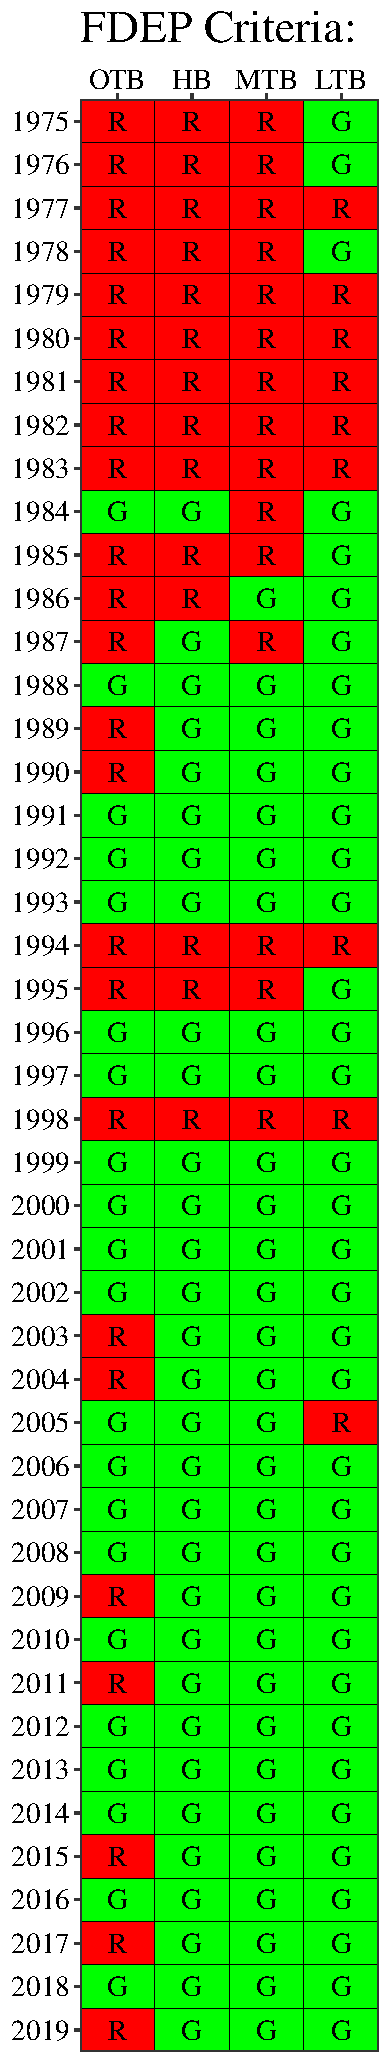
\includegraphics[trim = 0cm 0cm 0cm 0cm, width=1.1\linewidth]{figure/chlmat.pdf}}
\caption{\footnotesize Attainment of bay segments for chlorophyll criteria from 1975 to 2019.}
\label{fig:chlmat}
\end{figure}

\end{column}

%%%%%%%%%%%%%%
% right
%%%%%%%%%%%%%%    
\begin{column}{.65\linewidth}

\begin{block}{Maintaining Reasonable Assurance \& TMDL Compliance}
\footnotesize
In November 2017, the Florida Department of Environmental Protection (FDEP) accepted the 2017 Reasonable Assurance Update (2017 RA Update) as submitted by TBEP in partnership with the Tampa Bay Nitrogen Management Consortium. FDEP concluded that the RA Update demonstrated both attainment of seagrass targets and total nitrogen numeric criteria for 2012-2016. During 2019, all bay segments, excluding Old Tampa Bay, were in compliance with the FDEP regulatory criteria for chlorophyll-a concentrations (Figure \ref{fig:chlmat}). The second compliance report for the 2017-2021 period was submitted March 2019. 
\end{block}

\begin{block}{2019 Chl-a Monthly Variation Compared to 1974-2018}
\footnotesize
Chlorophyll-a concentrations were evaluated within the bay on a monthly basis during 2019 and compared to prior years' levels (Figure \ref{fig:chlboxplot}). Elevated concentrations in Old Tampa Bay were primarily due to \textit{Pyrodinium bahamense}. Lower Tampa Bay also showed elevated concentrations in August.
\end{block}



\vspace{-0.1in}

\begin{figure}
\centerline{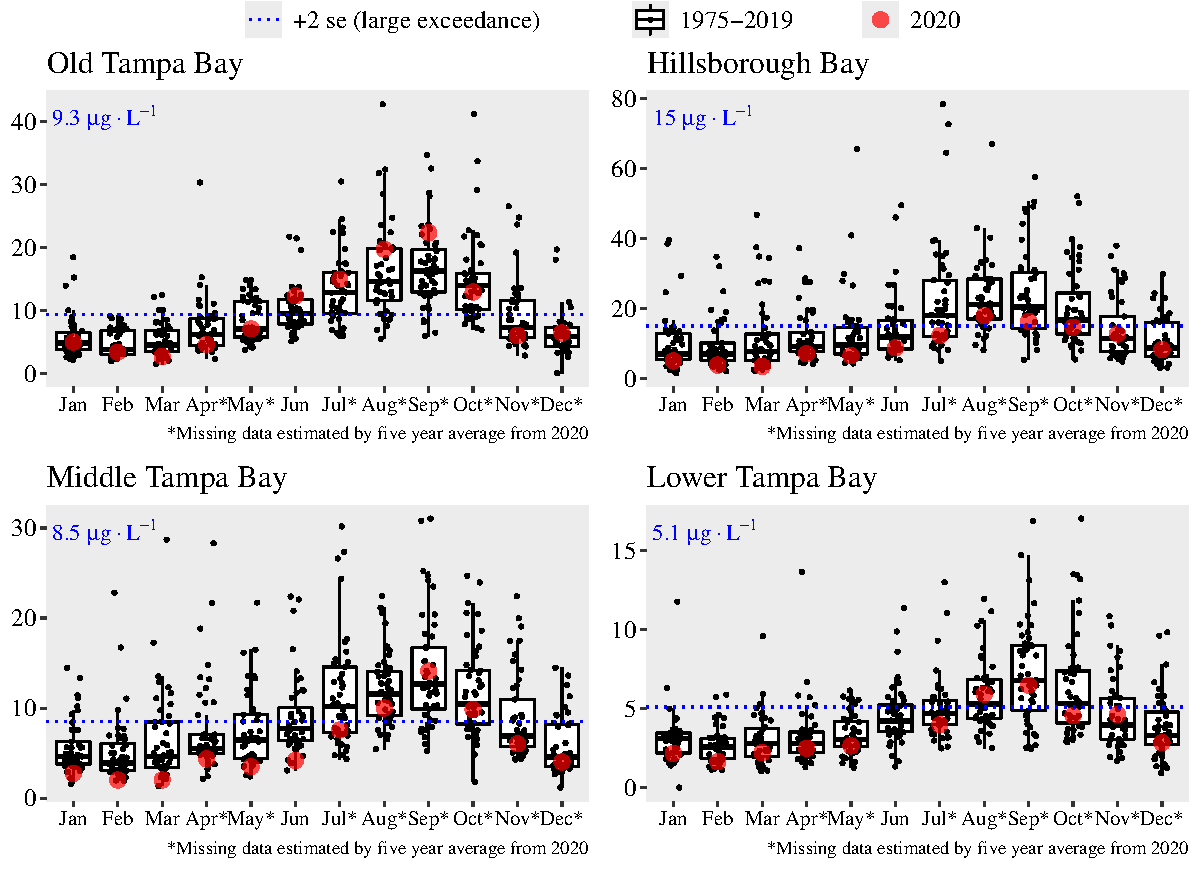
\includegraphics[trim = 0cm 0cm 0cm 0cm, width=1\linewidth]{figure/chlboxplot.pdf}}
\caption{\footnotesize Chlorophyll-a monthly averages from 1975-2018 for the four bay segments. The monthly averages for 2019 are shown in red.Historic chlorophyll-a annual averages for the four bay segments.}
\label{fig:chlboxplot}
\end{figure}

\vspace{-0.375in}

\begin{block}{Tampa Bay Seagrass Recovery}
\begin{minipage}{0.5\textwidth}
\footnotesize
Tampa Bay's total seagrass coverage remains above the recovery goal, though a slight decrease was observed from 2016 to 2018. The 2018 baywide coverage was estimated at 40,652 acres (Figure \ref{fig:sgtrnd}). As in 2016, coverage remains above the target (38,000 acres) and the estimated historic coverage of the 1950s (40,420 acres). The next SWFWMD coverage estimates will be developed from aerial photographs acquired over the winter 2019-20 period, following the extensive red tide event observed throughout 2018 (note: the 2018 coverage estimate was developed prior this event). More information can be found in TBEP technical publication \href{(https://tbeptech.org/TBEP_TECH_PUBS/2016/TBEP_08_16_2016_Seagrass_Transect_Summary_Report.pdf}{\#08-16} and \href{https://www.tbeptech.org/TBEP_TECH_PUBS/2017/TBEP_09_17_Sherwood_et_al_TB_Seagrass_SE_Geographer_project_muse_667989.pdf}{\#09-17}.
\end{minipage}
\hspace{0.01in}
\begin{minipage}{0.45\textwidth}
\begin{figure}
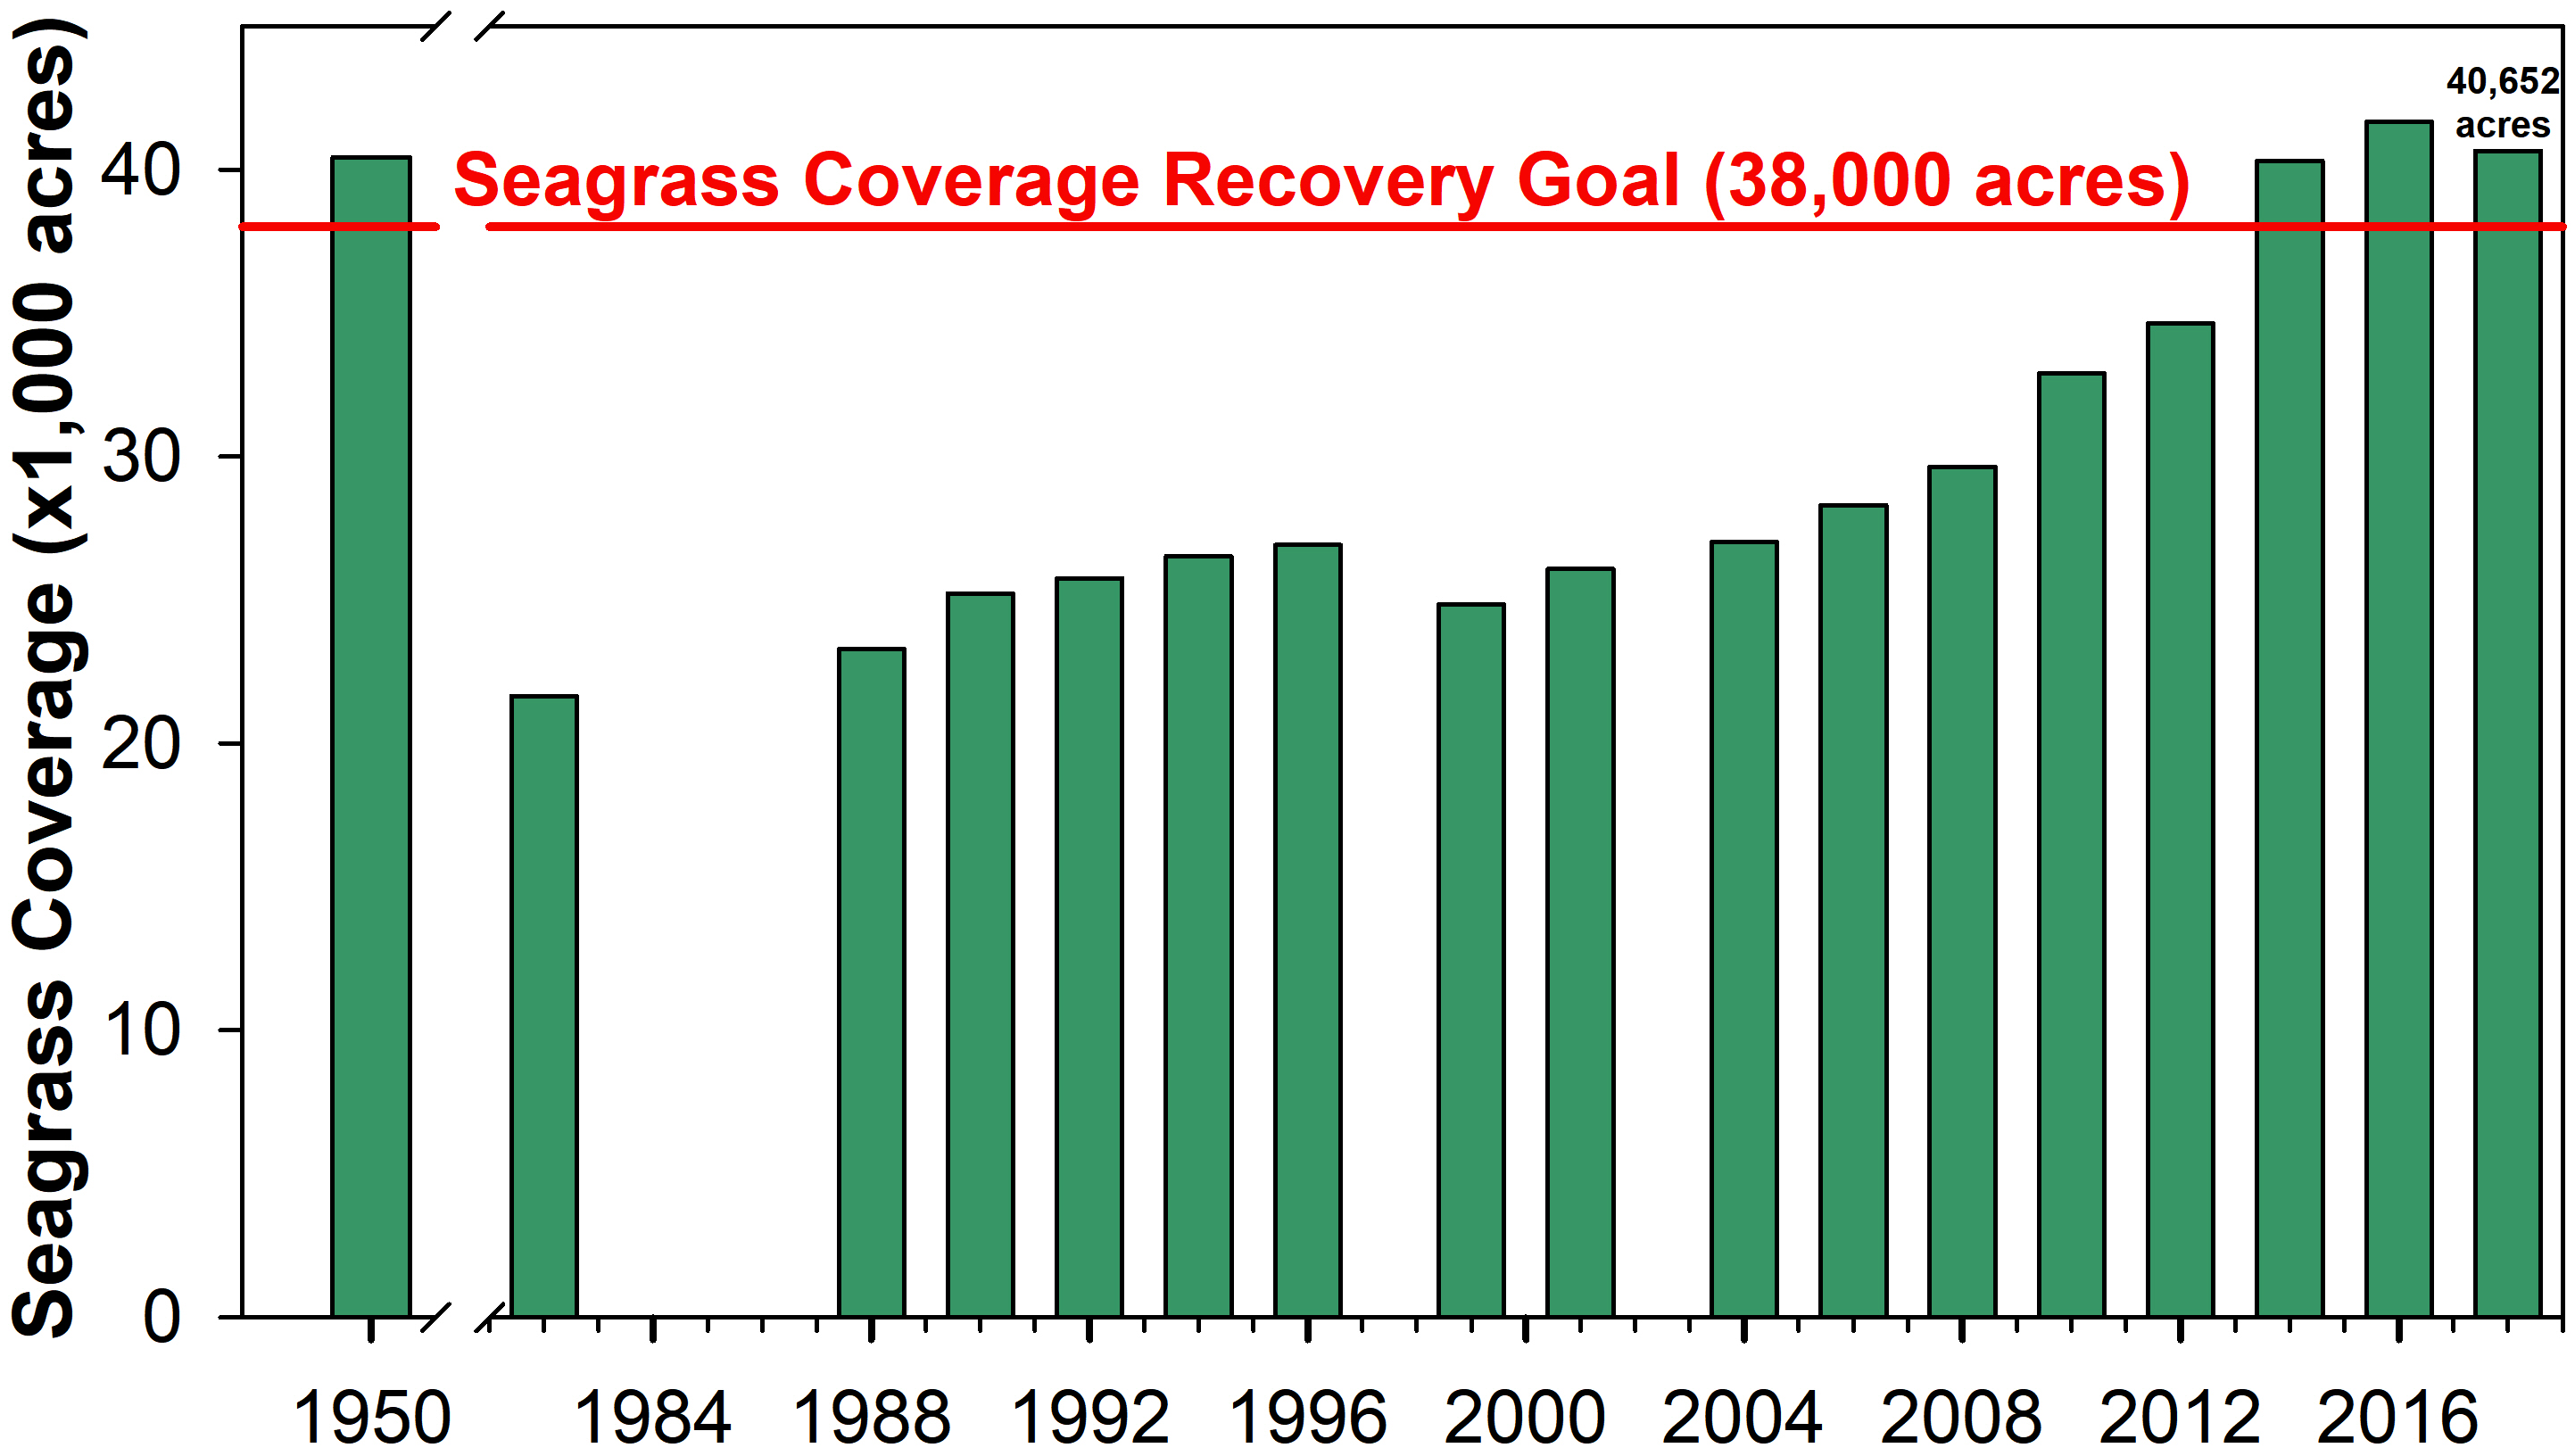
\includegraphics[width=\textwidth, trim = 0cm 0cm 0cm -1cm]{www/Seagrass_Acreage_1950_2018.png}
\caption{\footnotesize Historic seagrass acreage estimates for Tampa Bay from 1950-2018 (Source: TBEP \& SWFWMD)}
\label{fig:sgtrnd}
\end{figure}
\end{minipage}
\end{block}

\vspace{0.1in}

\footnotesize \textit{\textbf{Additional info}: 2019 nutrient management compliance assessment available from Sherwood, E., Burke, M. 2019. \href{http://www.tbeptech.org/TBEP_TECH_PUBS/2019/TBEP_11-19_TBNMC_2018_RA_Annual_Assessment.pdf}{TBEP Technical Report \#11-19}.} \\

\end{column}

\end{columns}

\end{frame}

\end{document}
